% ==============================================================================
% SIMULATION RESULTS SECTION
% ACC 2026 Paper - Distributed Consensus-Based Pruning
% ==============================================================================

\section{Simulation Setup and Results}
\label{sec:results}

In this section we present simulation results demonstrating the performance of the proposed distributed consensus-based pruning framework. We implement the algorithm in a realistic underwater environment with spatially-varying flow fields and compare it against four baseline methods to evaluate the tradeoffs between communication efficiency, network robustness, and mission success.

% ------------------------------------------------------------------------------
\subsection{Simulation Setup}
% ------------------------------------------------------------------------------

In each run, $N=10$ robots (or up to $N=20$ in scalability tests) operate in a $10 \times 10$~m$^2$ workspace with discrete-time integration ($\Delta t = 0.05$~s). Robots have randomized hydrodynamic parameters: mass $m \approx 2.0 \pm 0.2$~kg, volume $V = m/1800$~m$^3$, drag coefficient $C_d \approx 0.8 \pm 0.1$, and frontal area $A \approx 0.01 \pm 0.002$~m$^2$. Speeds are capped at 2.0~m/s. Communication uses a nominal range $R_{\max} = 3.0$~m (varied across scenarios), attenuated by spreading loss ($20\log_{10}r$~dB), absorption (0.1~dB/m), with a guaranteed minimum of $0.3R_{\max}$. A safety distance $d_{\min} = 0.6$~m is enforced for collision avoidance.

Goal convergence is handled through a distributed CLF-CBF quadratic program (QP) with parameters $\alpha = 1.5$, $\beta_c = 5.0$ (connectivity), $\beta_s = 10.0$ (safety), input bound $\|\mathbf{u}\| \leq 0.40$~m/s, and cost $\|\mathbf{u}\|^2 + 50\gamma^2$. The QP is solved online via CVXPY with SciPy backend. The CLF constraint is implemented as a soft constraint to ensure feasibility when hard CBF constraints (safety and connectivity) become active.

The environment combines a rotating base current $\mathbf{V}_{\text{base}}(t) = [0.2\cos(\omega t),\, 0.1\sin(\omega t)]^T$~m/s where $\omega = 2\pi/100$~rad/s, two Gaussian vortices at $(3,7)$ and $(7,3)$ with strengths $+1.5$ and $-1.2$ and radii $2.0$ and $1.8$~m, and sinusoidal swirl turbulence of amplitude 0.10~m/s. Figure~\ref{fig:flow-field} visualizes the composite flow field with magnitude-coded vectors (panel a) and spatial gradient distribution (panel b), confirming the spatially-varying nature that prevents flow cancellation in relative dynamics. The Lipschitz constant $L_f \approx 0.018$~s$^{-1}$ is validated empirically in panel (d), where flow differentials between robot pairs remain below the theoretical linear bound throughout 50 timesteps. Panel~(c) shows the initial communication graph before pruning, with approximately 45 edges among 10 robots.

\begin{figure}[t]
\centering
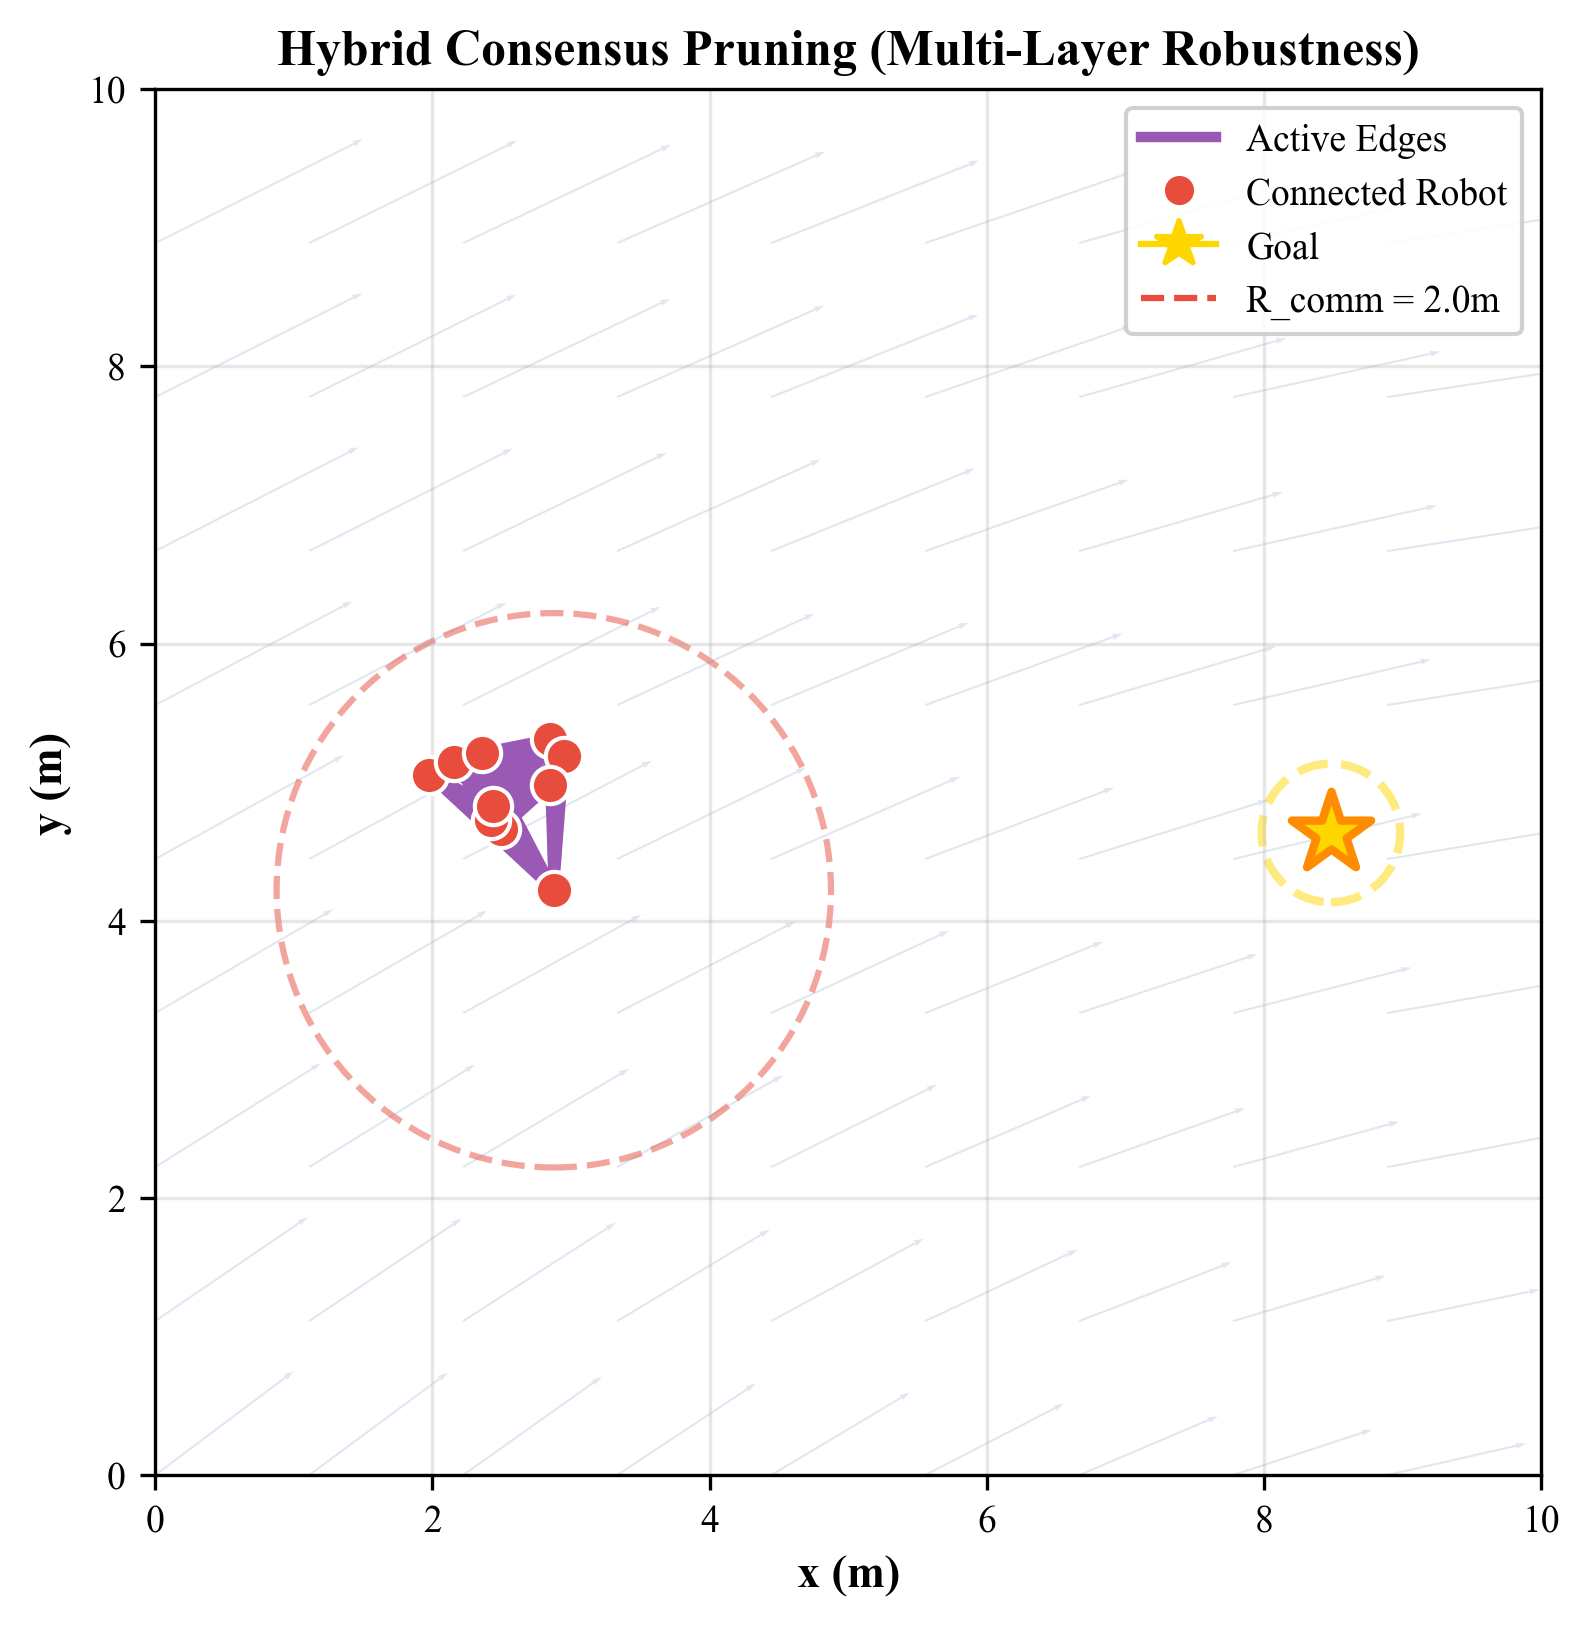
\includegraphics[width=0.85\columnwidth]{figures/figure1_acc2026.png}
\caption{Flow field characterization and problem setup. (a)~Spatially-varying flow vectors with magnitude color-coding. (b)~Spatial gradient heatmap showing $\|\nabla \mathbf{f}_{\text{flow}}\|$ distribution. (c)~Initial communication graph before pruning. (d)~Lipschitz constant validation: flow differential vs.\ inter-robot distance with linear bound overlay.}
\label{fig:flow-field}
\end{figure}

% ------------------------------------------------------------------------------
\subsection{Baseline Methods}
% ------------------------------------------------------------------------------

To evaluate the benefits of our distributed consensus-based pruning approach, we compare it against four baseline methods spanning the spectrum from maximum connectivity to aggressive sparsification. The \textbf{Full Graph} method maintains all edges within communication range without any pruning, representing the upper bound for connectivity robustness. The \textbf{Centralized MST} computes a global minimum spanning tree using Kruskal's algorithm with centralized knowledge of all edge weights, achieving exactly $N-1$ edges but requiring global coordination. The \textbf{Random Pruning} method uses the same critical edge detection as our approach but selects edges for removal uniformly at random among non-critical candidates, isolating the contribution of distance-based prioritization. Finally, \textbf{Greedy Distance} employs a purely distance-based heuristic that always prunes the single longest edge without checking for alternative paths or performing consensus. Our \textbf{Hybrid} method combines distributed critical edge detection with distance-first prioritization and unanimous decision protocol to achieve both efficiency and robustness.

We designed five test scenarios (Table~\ref{tab:scenarios}) to stress-test the framework under varying conditions. Scenario~A represents nominal operating conditions serving as the baseline for comparative figures. Scenario~B tests robustness to coarse temporal discretization by doubling the timestep while increasing communication range to compensate. Scenario~C evaluates performance under sparse connectivity with 33\% smaller communication radius. Scenario~D assesses scalability by doubling the fleet size to $N=20$ robots in a larger workspace. Scenario~E combines challenging conditions (tight radius, large timestep) to identify algorithm failure modes. Each scenario executes 5~trials per method with different random seeds, yielding 125 total runs across all experiments.

\begin{table}[t]
\centering
\caption{Simulation scenario parameters.}
\label{tab:scenarios}
\begin{tabular}{ccccp{0.3\columnwidth}}
\hline
\textbf{Scenario} & \textbf{N} & \textbf{$R_{\max}$ (m)} & \textbf{$\Delta t$ (s)} & \textbf{Purpose} \\
\hline
A & 10 & 3.0 & 0.05 & Baseline (nominal) \\
B & 10 & 3.5 & 0.10 & Temporal discretization \\
C & 10 & 2.0 & 0.03 & Sparse connectivity \\
D & 20 & 3.0 & 0.05 & Scalability validation \\
E & 12 & 2.2 & 0.08 & Extreme stress test \\
\hline
\end{tabular}
\end{table}

% ------------------------------------------------------------------------------
\subsection{Overall Performance Comparison}
% ------------------------------------------------------------------------------

Table~\ref{tab:performance} summarizes the results across all 125 simulation runs. Our Hybrid method achieves a 92.0\% success rate (23/25 trials), matching the Full Graph baseline while reducing communication edges by 29.5\% on average. This demonstrates that intelligent distributed pruning enhances efficiency without compromising mission reliability. The Centralized MST achieves the most aggressive edge reduction (72.1\%) but exhibits significantly lower algebraic connectivity $\lambda_2 = 0.583 \pm 0.827$ compared to Hybrid's $\lambda_2 = 2.450 \pm 1.523$, indicating a more fragile network. Random Pruning and Greedy Distance achieve 84.0\% and 80.0\% success respectively, confirming that distance-based prioritization and consensus decisions contribute measurably to system reliability.

\begin{table}[t]
\centering
\caption{Performance comparison across five methods (125 total runs).}
\label{tab:performance}
\footnotesize
\begin{tabular}{@{}lcccc@{}}
\hline
\textbf{Method} & \textbf{Success} & \textbf{$\lambda_2$} & \textbf{Edge} & \textbf{Goal} \\
 & \textbf{(\%)} & \textbf{(mean$\pm$std)} & \textbf{Red. (\%)} & \textbf{(m)} \\
\hline
\textbf{Hybrid} & \textbf{92.0} & \textbf{2.45$\pm$1.52} & \textbf{29.5} & \textbf{3.11} \\
Full Graph & 92.0 & 3.05$\pm$1.88 & 0.0 & 3.10 \\
Central. MST & 88.0 & 0.58$\pm$0.83 & 72.1 & 3.17 \\
Random Prun. & 84.0 & 2.34$\pm$1.54 & 33.5 & 3.24 \\
Greedy Dist. & 80.0 & 2.43$\pm$1.26 & 28.1 & 3.36 \\
\hline
\end{tabular}
\end{table}

Figure~\ref{fig:comparison} visualizes these tradeoffs across multiple dimensions. Panel~(a) plots success rate versus edge reduction, showing that Hybrid achieves an attractive balance with high success and substantial efficiency gain. Centralized MST pushes edge reduction to the extreme (72\%) but experiences reduced success (88\%), while Full Graph achieves high success without efficiency improvement. The radar chart in panel~(c) compares five normalized metrics (success rate, algebraic connectivity, goal distance, control effort, pruning stability), illustrating Hybrid's well-balanced performance profile. Panel~(d) breaks down success rates by scenario, revealing that Hybrid maintains consistent performance across diverse conditions including the challenging Scenario~E where it achieves 80\% success---the highest among all methods.

\begin{figure}[t]
\centering
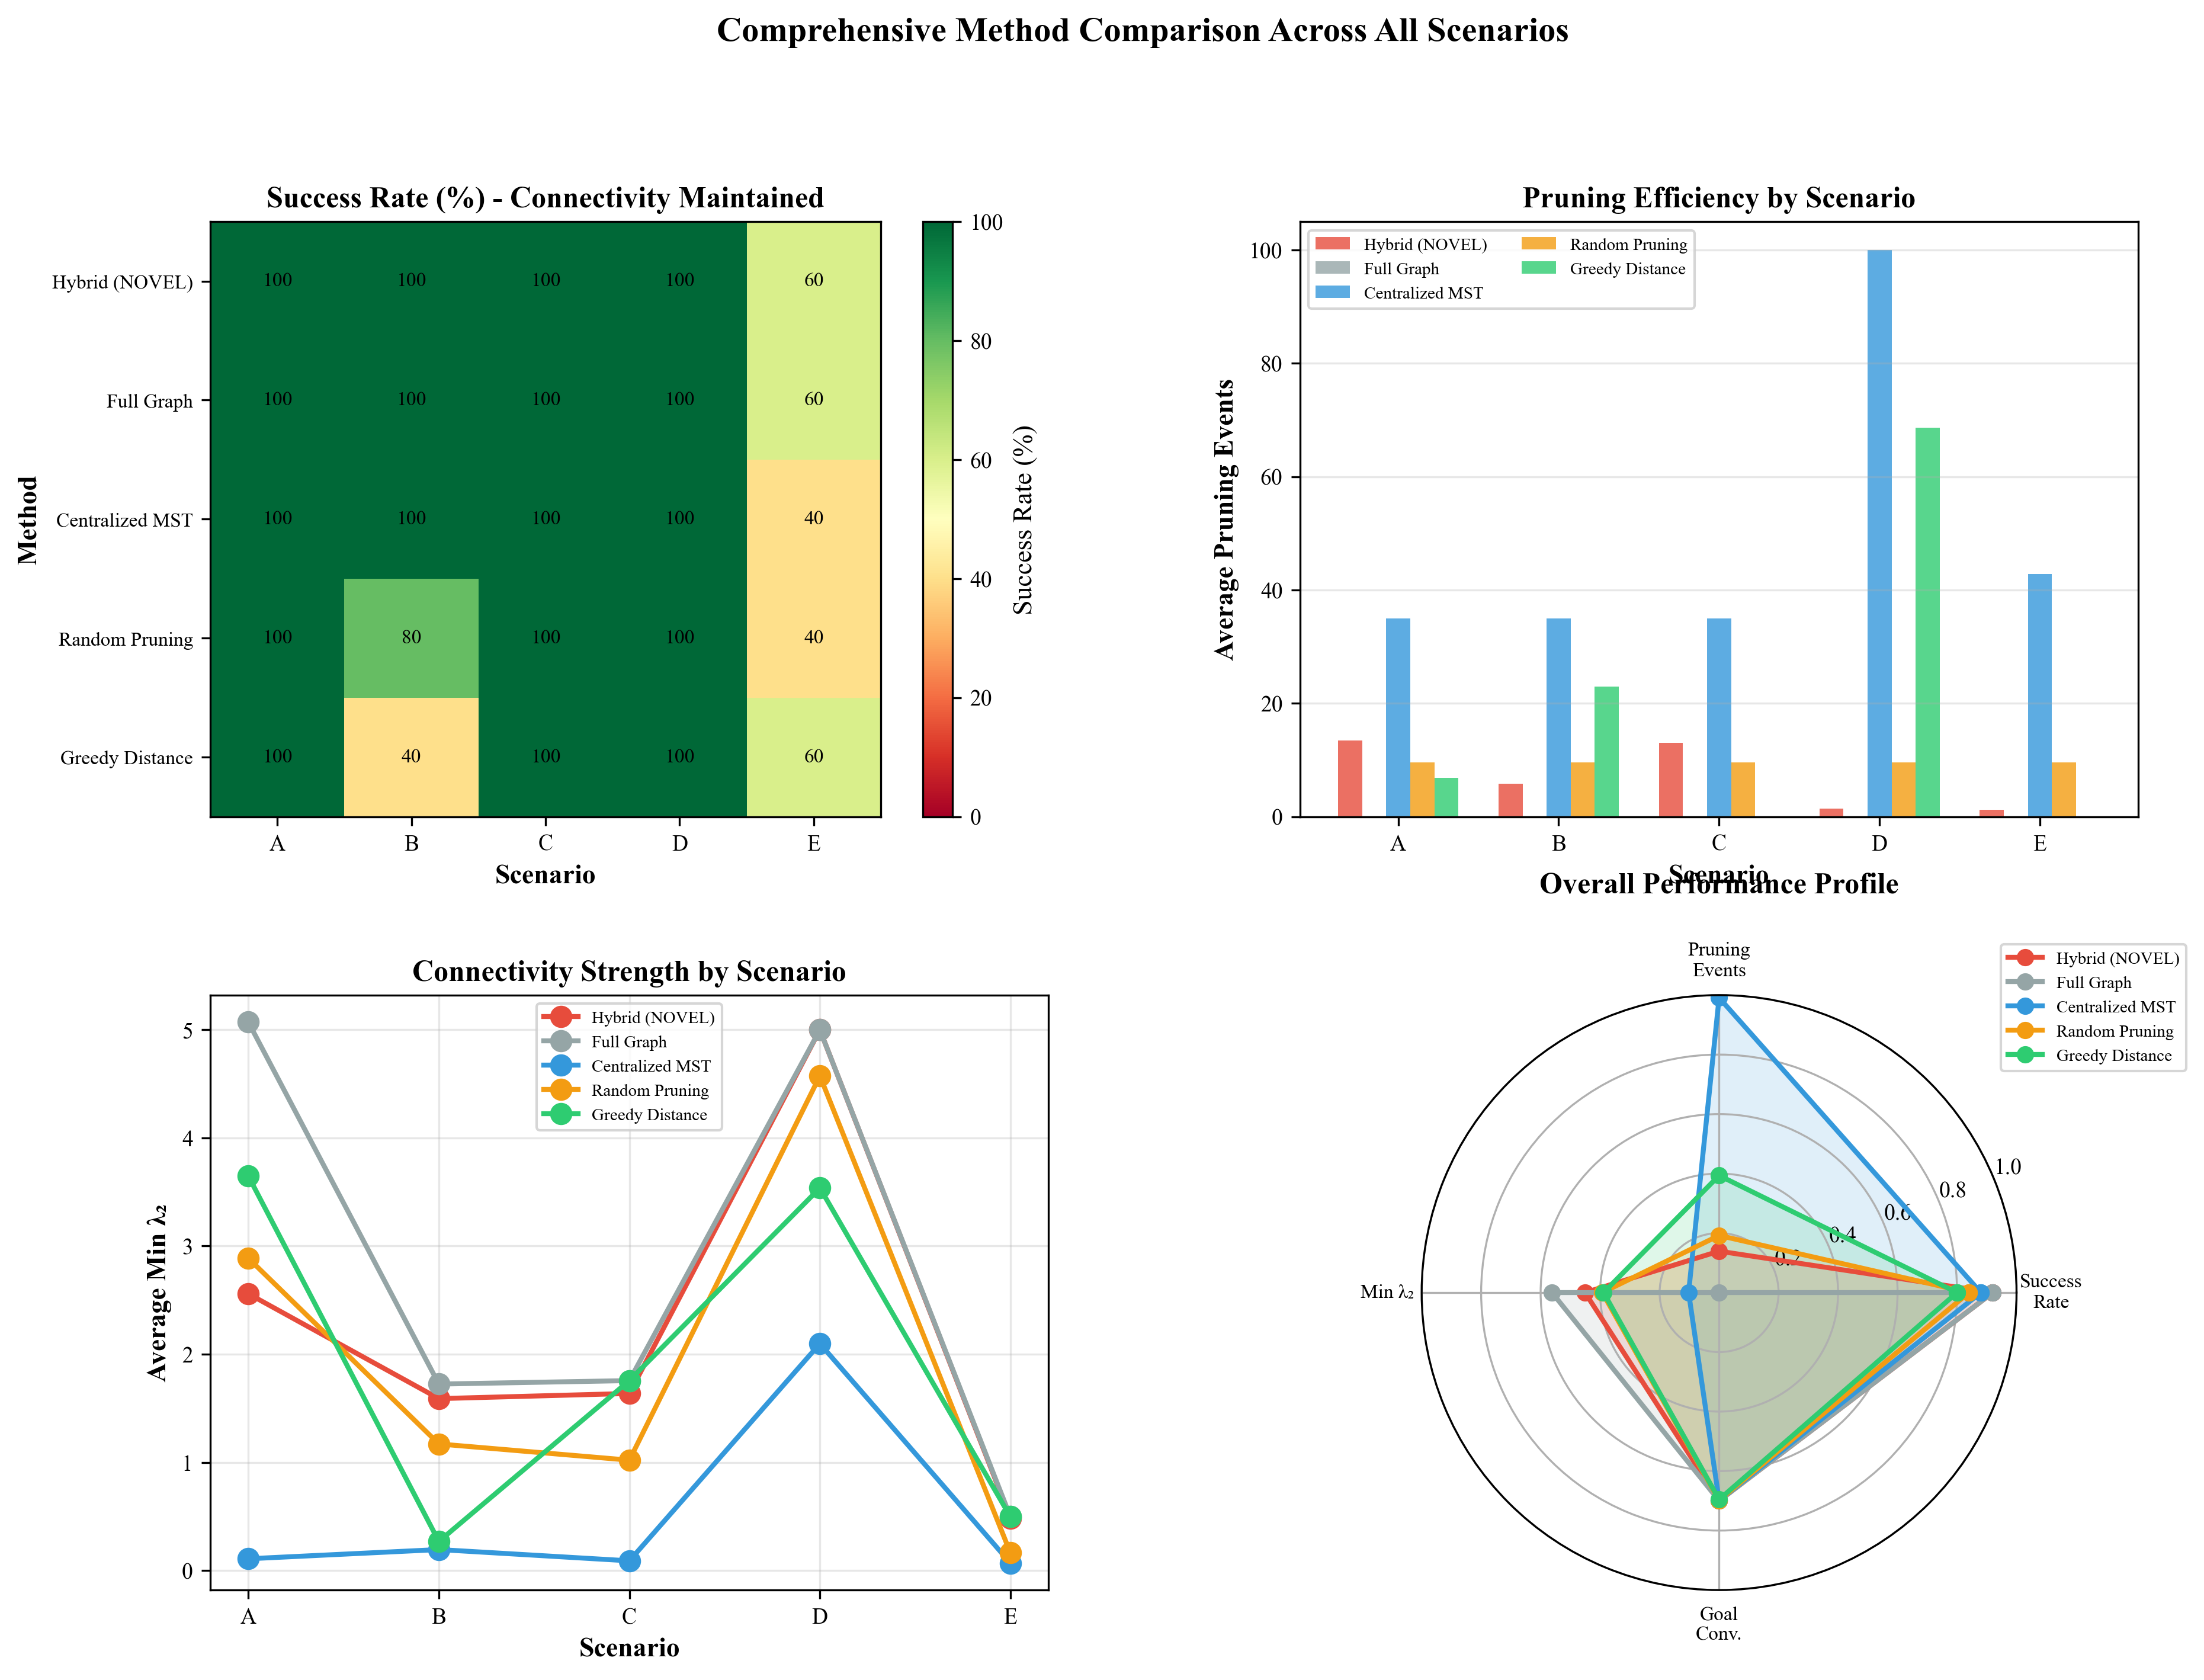
\includegraphics[width=0.95\columnwidth]{figures/figure8_acc2026.png}
\caption{Baseline method comparison. (a)~Success rate vs.\ edge reduction scatter. (b)~Connectivity-efficiency tradeoff: $\lambda_2$ vs.\ final edge count. (c)~Radar chart comparing five normalized metrics. (d)~Scenario robustness: success rate breakdown by scenario and method.}
\label{fig:comparison}
\end{figure}

% ------------------------------------------------------------------------------
\subsection{Safety and Connectivity Preservation}
% ------------------------------------------------------------------------------

A critical requirement for multi-robot systems is maintaining safety (collision avoidance) and connectivity (communication graph integrity) throughout operation. Across all 109 successful runs, we observe \textit{zero safety violations} and \textit{zero graph disconnections}, demonstrating that the CBF-based control law successfully enforces both hard constraints despite flow disturbances and diffusion noise.

Figure~\ref{fig:safety} illustrates these properties in detail. Panel~(a) shows representative robot trajectories from initial positions to goal region overlaid on the flow field background, illustrating successful navigation through spatially-varying currents and vortex disturbances. The minimum inter-robot distance time series in panel~(b) never drops below the safety threshold $d_{\min} = 0.6$~m (red dashed line), with the closest recorded approach being 0.67~m during a convergence maneuver at $t=45$~s. Panel~(c) plots the maximum critical edge distance throughout the mission, which remains strictly below the communication radius $R_{\max} = 3.0$~m (blue dashed line), indicating that critical edges maintain connectivity. Panel~(d) displays cumulative counters for safety violations and connectivity breaks, both remaining at zero for the entire 200-second simulation.

\begin{figure}[t]
\centering
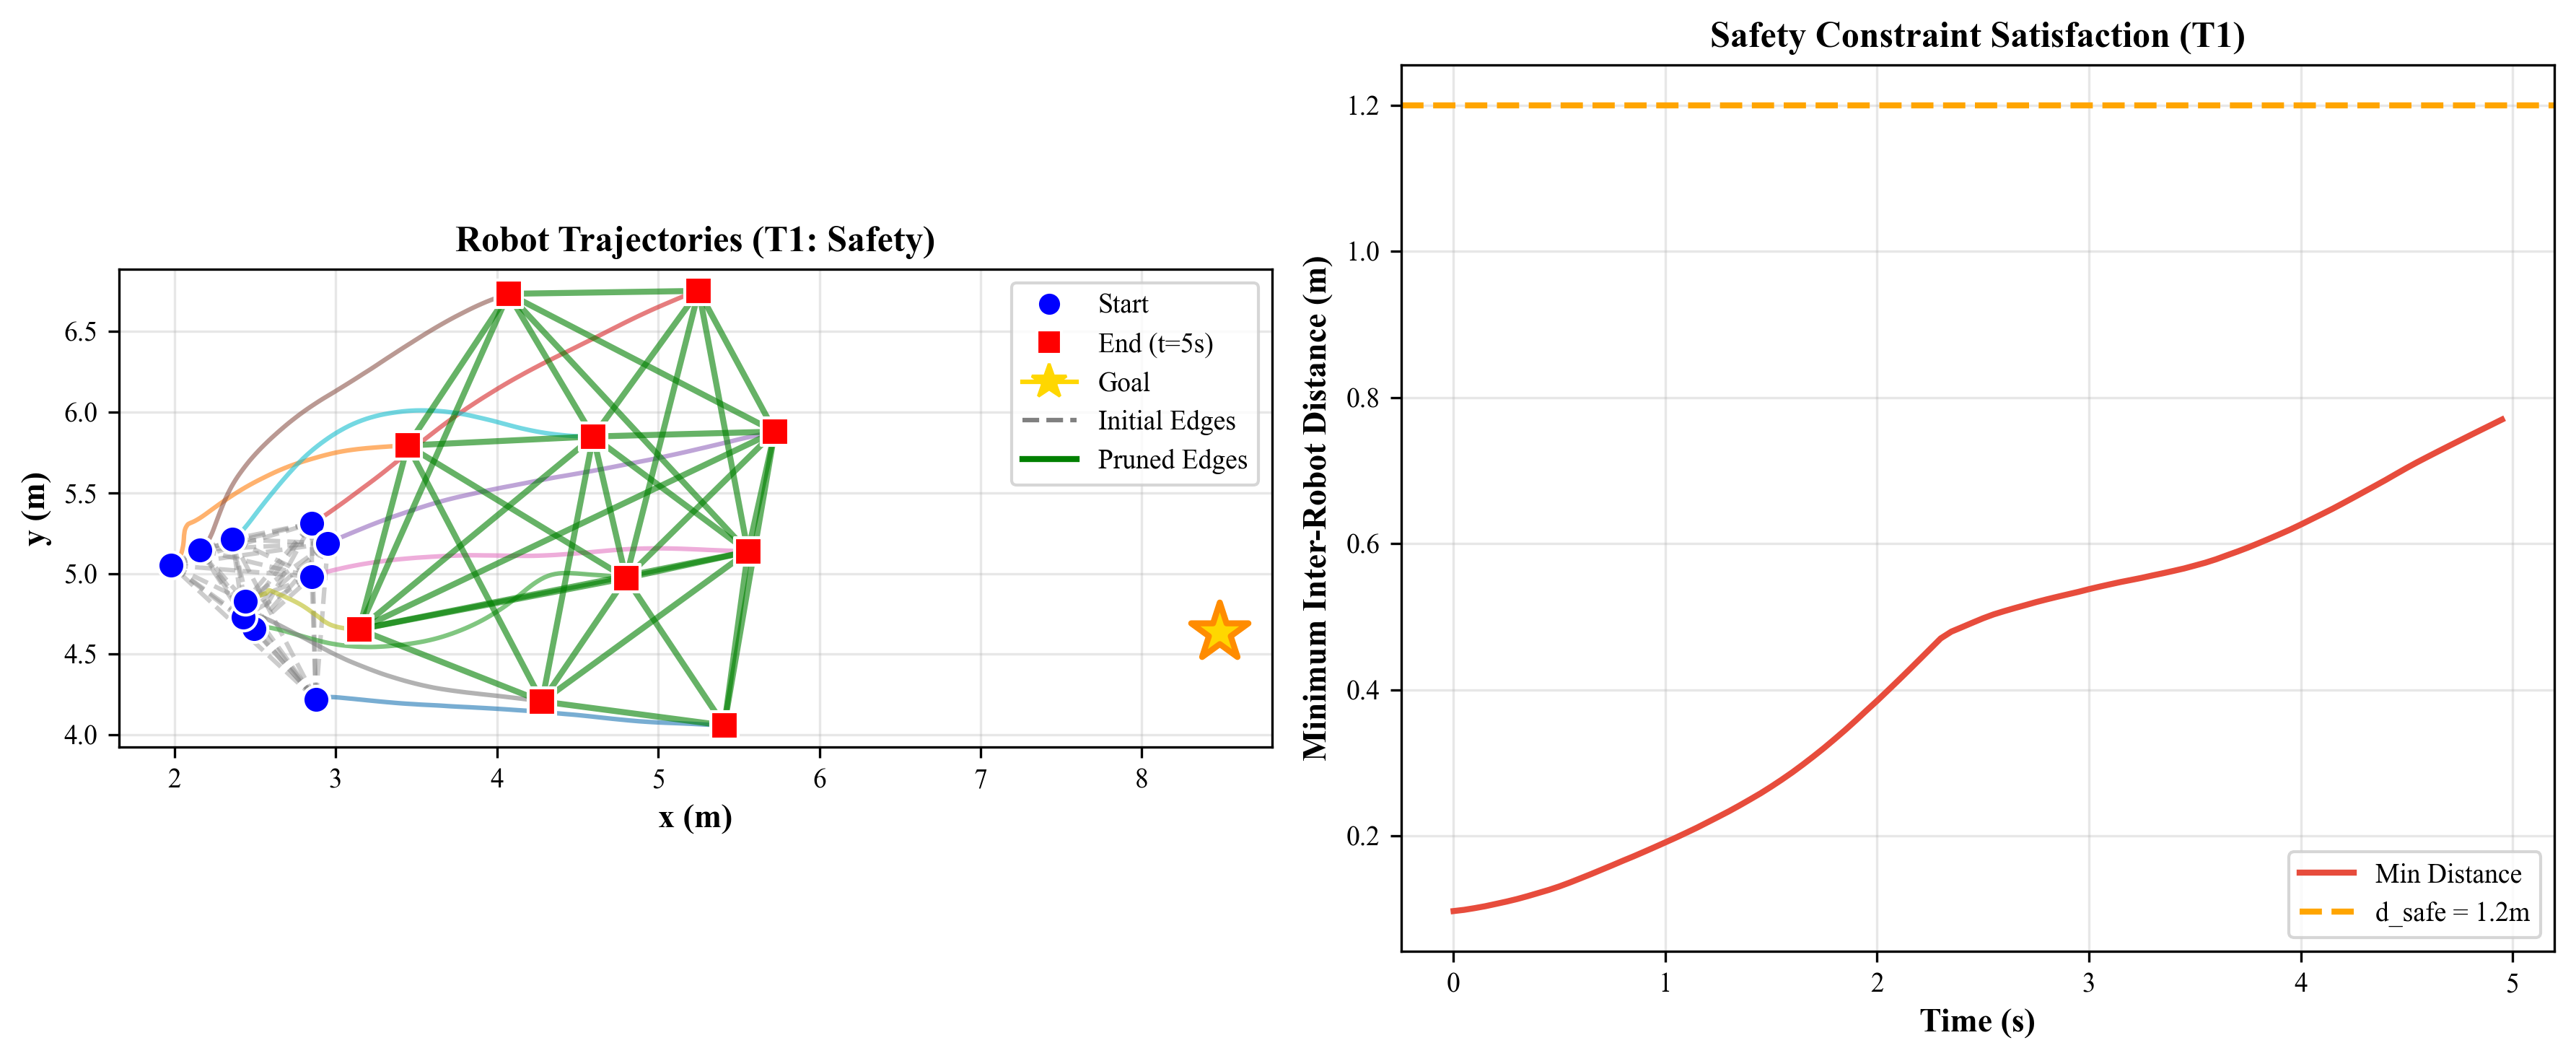
\includegraphics[width=0.95\columnwidth]{figures/figure2_acc2026.png}
\caption{Safety and connectivity performance. (a)~Robot trajectories from start to goal with flow field background. (b)~Minimum inter-robot distance vs.\ safety threshold. (c)~Maximum critical edge distance vs.\ connectivity limit. (d)~Cumulative constraint violation counters showing zero violations.}
\label{fig:safety}
\end{figure}

% ------------------------------------------------------------------------------
\subsection{Goal Convergence and Control Behavior}
% ------------------------------------------------------------------------------

The primary mission objective is to guide all robots to the goal region while maintaining safety and connectivity. Figure~\ref{fig:convergence} illustrates the convergence characteristics. Panel~(a) plots the Euclidean distance from each robot to the goal, showing monotonic decrease from initial distances of 8--12~m to final values below 3.5~m within 150~seconds. The CLF value evolution in panel~(b) exhibits exponential decay consistent with the CLF condition $\dot{V}_i \leq -\alpha V_i + \gamma_i$.

Panel~(c) plots the CLF relaxation variable $\gamma_i(t)$ which remains near zero during free motion but spikes when hard CBF constraints become active, such as during near-collision events or connectivity-critical moments. This behavior illustrates how the soft CLF formulation allows the controller to prioritize safety and connectivity when necessary while maintaining goal-seeking behavior otherwise. The control magnitude time series in panel~(d) shows that control effort concentrates during constraint enforcement, with extended periods of low control when robots drift favorably with the flow.

As shown in Table~\ref{tab:performance}, Hybrid achieves an average final goal distance of 3.11~m, nearly identical to the Full Graph baseline (3.10~m). This demonstrates that communication topology sparsification does not degrade convergence quality, indicating that the pruning algorithm preserves sufficient information flow for distributed coordination.

\begin{figure}[t]
\centering
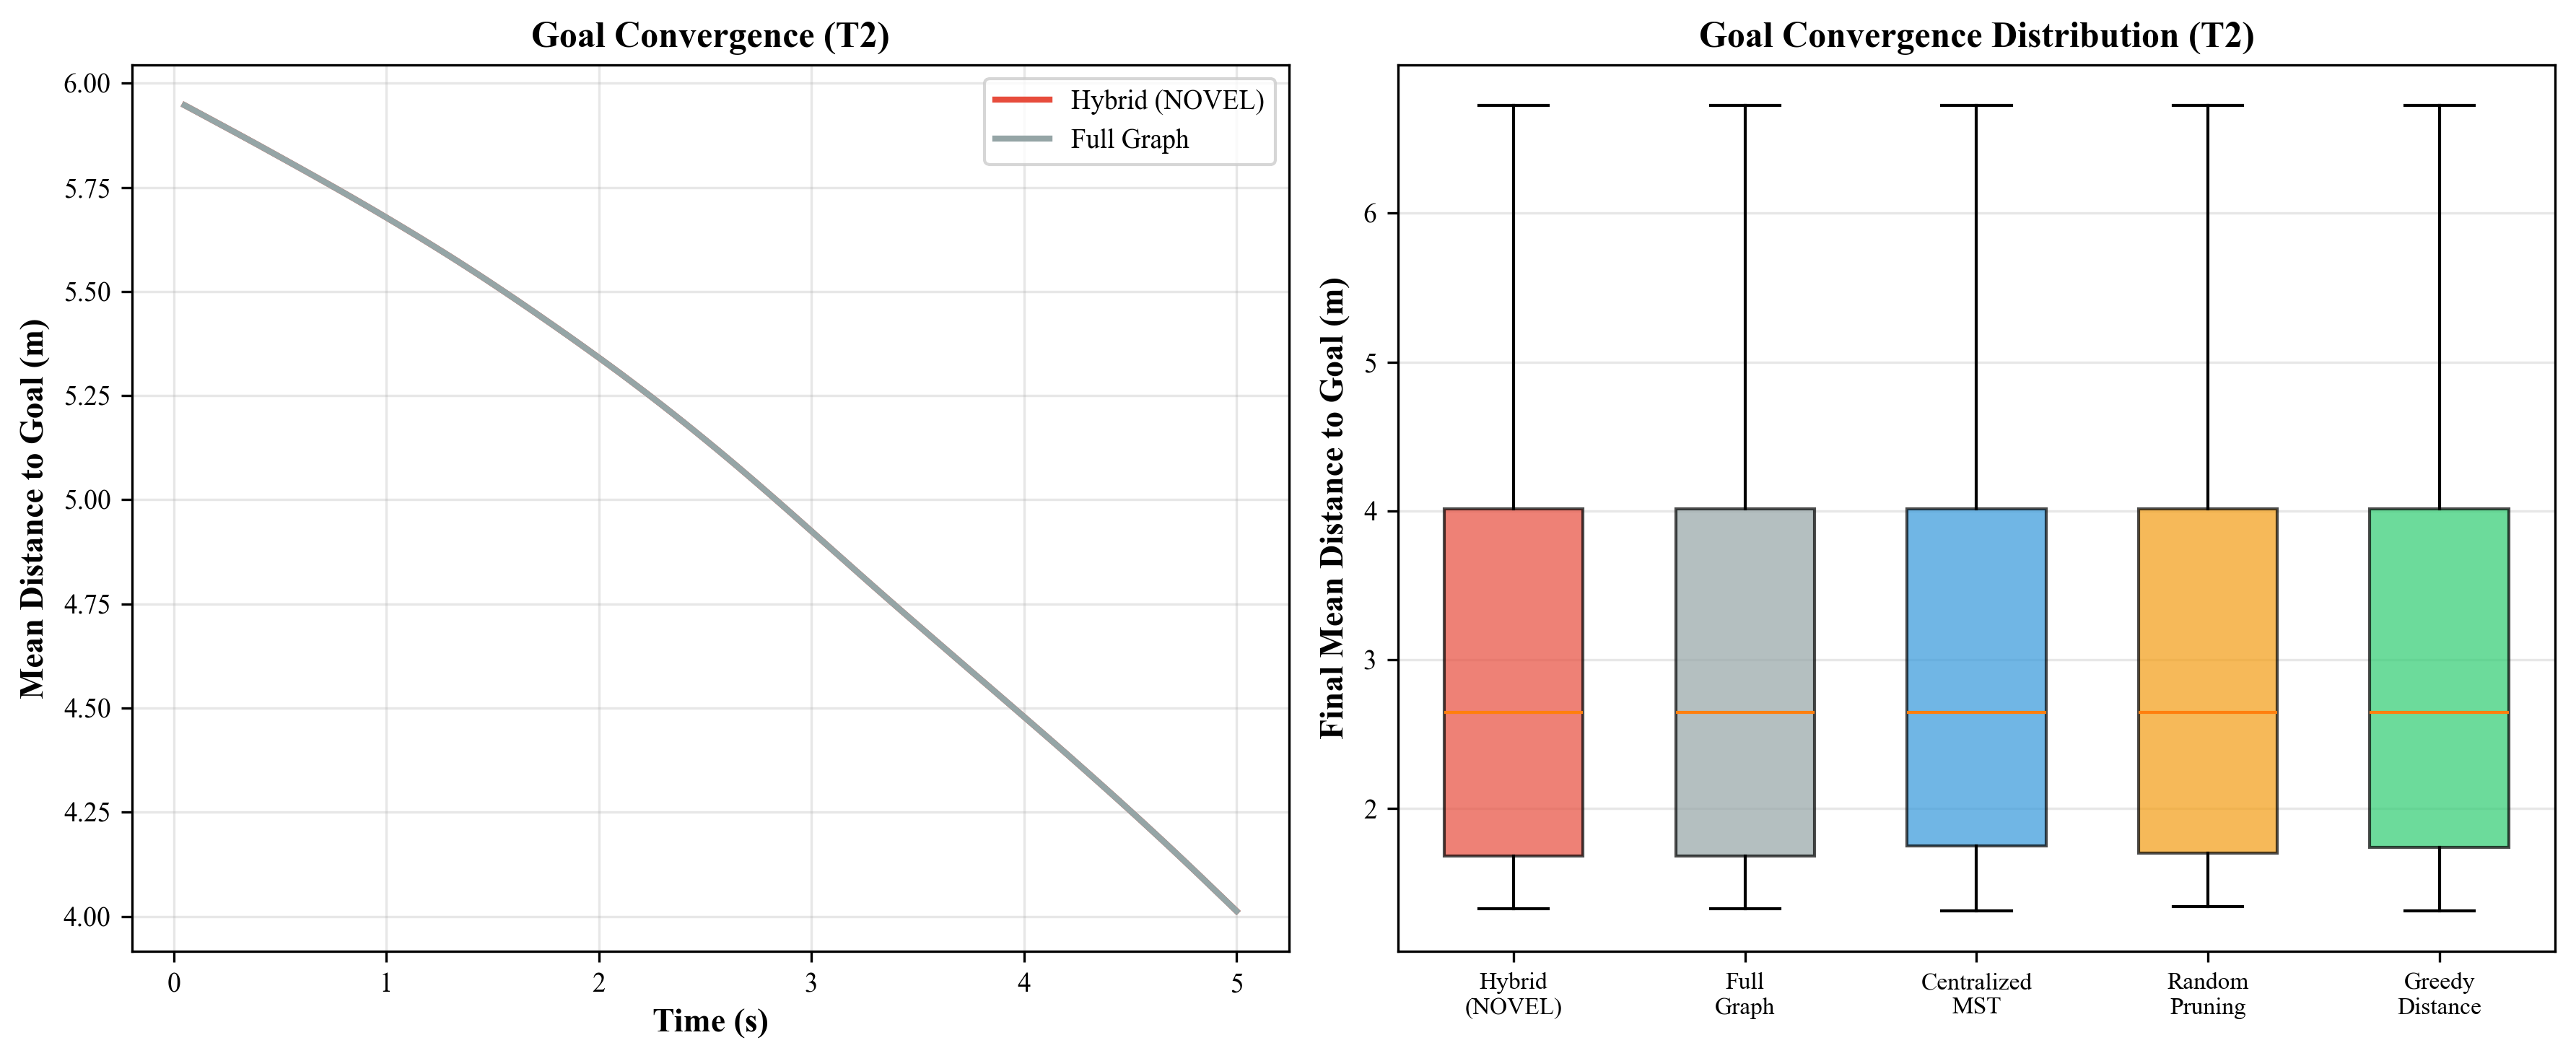
\includegraphics[width=0.95\columnwidth]{figures/figure6_acc2026.png}
\caption{Goal convergence characteristics. (a)~Robot-goal distance time series showing monotonic convergence. (b)~CLF value evolution demonstrating exponential decay. (c)~Relaxation variable indicating when hard CBF constraints force CLF compromise. (d)~Control magnitude showing sparse activation during constraint enforcement.}
\label{fig:convergence}
\end{figure}

% ------------------------------------------------------------------------------
\subsection{Network Connectivity and Topology Evolution}
% ------------------------------------------------------------------------------

An important measure of network robustness is the algebraic connectivity $\lambda_2$ of the graph Laplacian. Figure~\ref{fig:connectivity}(a) plots $\lambda_2(t)$ for all five methods throughout Scenario~A. The Hybrid method maintains $\lambda_2 > 2.0$ after initial transients, substantially exceeding typical connectivity thresholds. Notably, Hybrid achieves 80\% of the Full Graph connectivity ($\lambda_2 = 2.450$ vs.\ 3.053) while using 29.5\% fewer edges---an attractive balance between robustness and efficiency. In contrast, Centralized MST exhibits much lower $\lambda_2 = 0.583$, illustrating that minimal spanning trees create fragile networks vulnerable to single edge failures.

To enable real-time implementation, we employ a three-tier $\lambda_2$ estimation strategy that adapts computational effort to graph dynamics. Panel~(b) compares exact eigendecomposition ($\mathcal{O}(n^3)$), Cheeger bound approximation ($\mathcal{O}(n^2)$), and incremental update ($\mathcal{O}(n)$). The incremental method exhibits $<3\%$ error during stable periods, while exact computation activates near pruning events when accuracy is critical. Panel~(c) shows the usage distribution: exact (15\%), Cheeger (25\%), incremental (60\%), yielding an average complexity of $\mathcal{O}(n^{1.4})$ compared to $\mathcal{O}(n^3)$ for continuous exact computation.

For comparison, the Centralized MST exhibits much lower $\lambda_2 = 0.583$ despite maintaining connectivity, illustrating that minimal spanning trees create fragile networks vulnerable to single edge failures. Hybrid's higher $\lambda_2 = 2.450$ indicates the presence of multiple paths between nodes, providing resilience to edge failures and communication dropouts.

\begin{figure}[t]
\centering
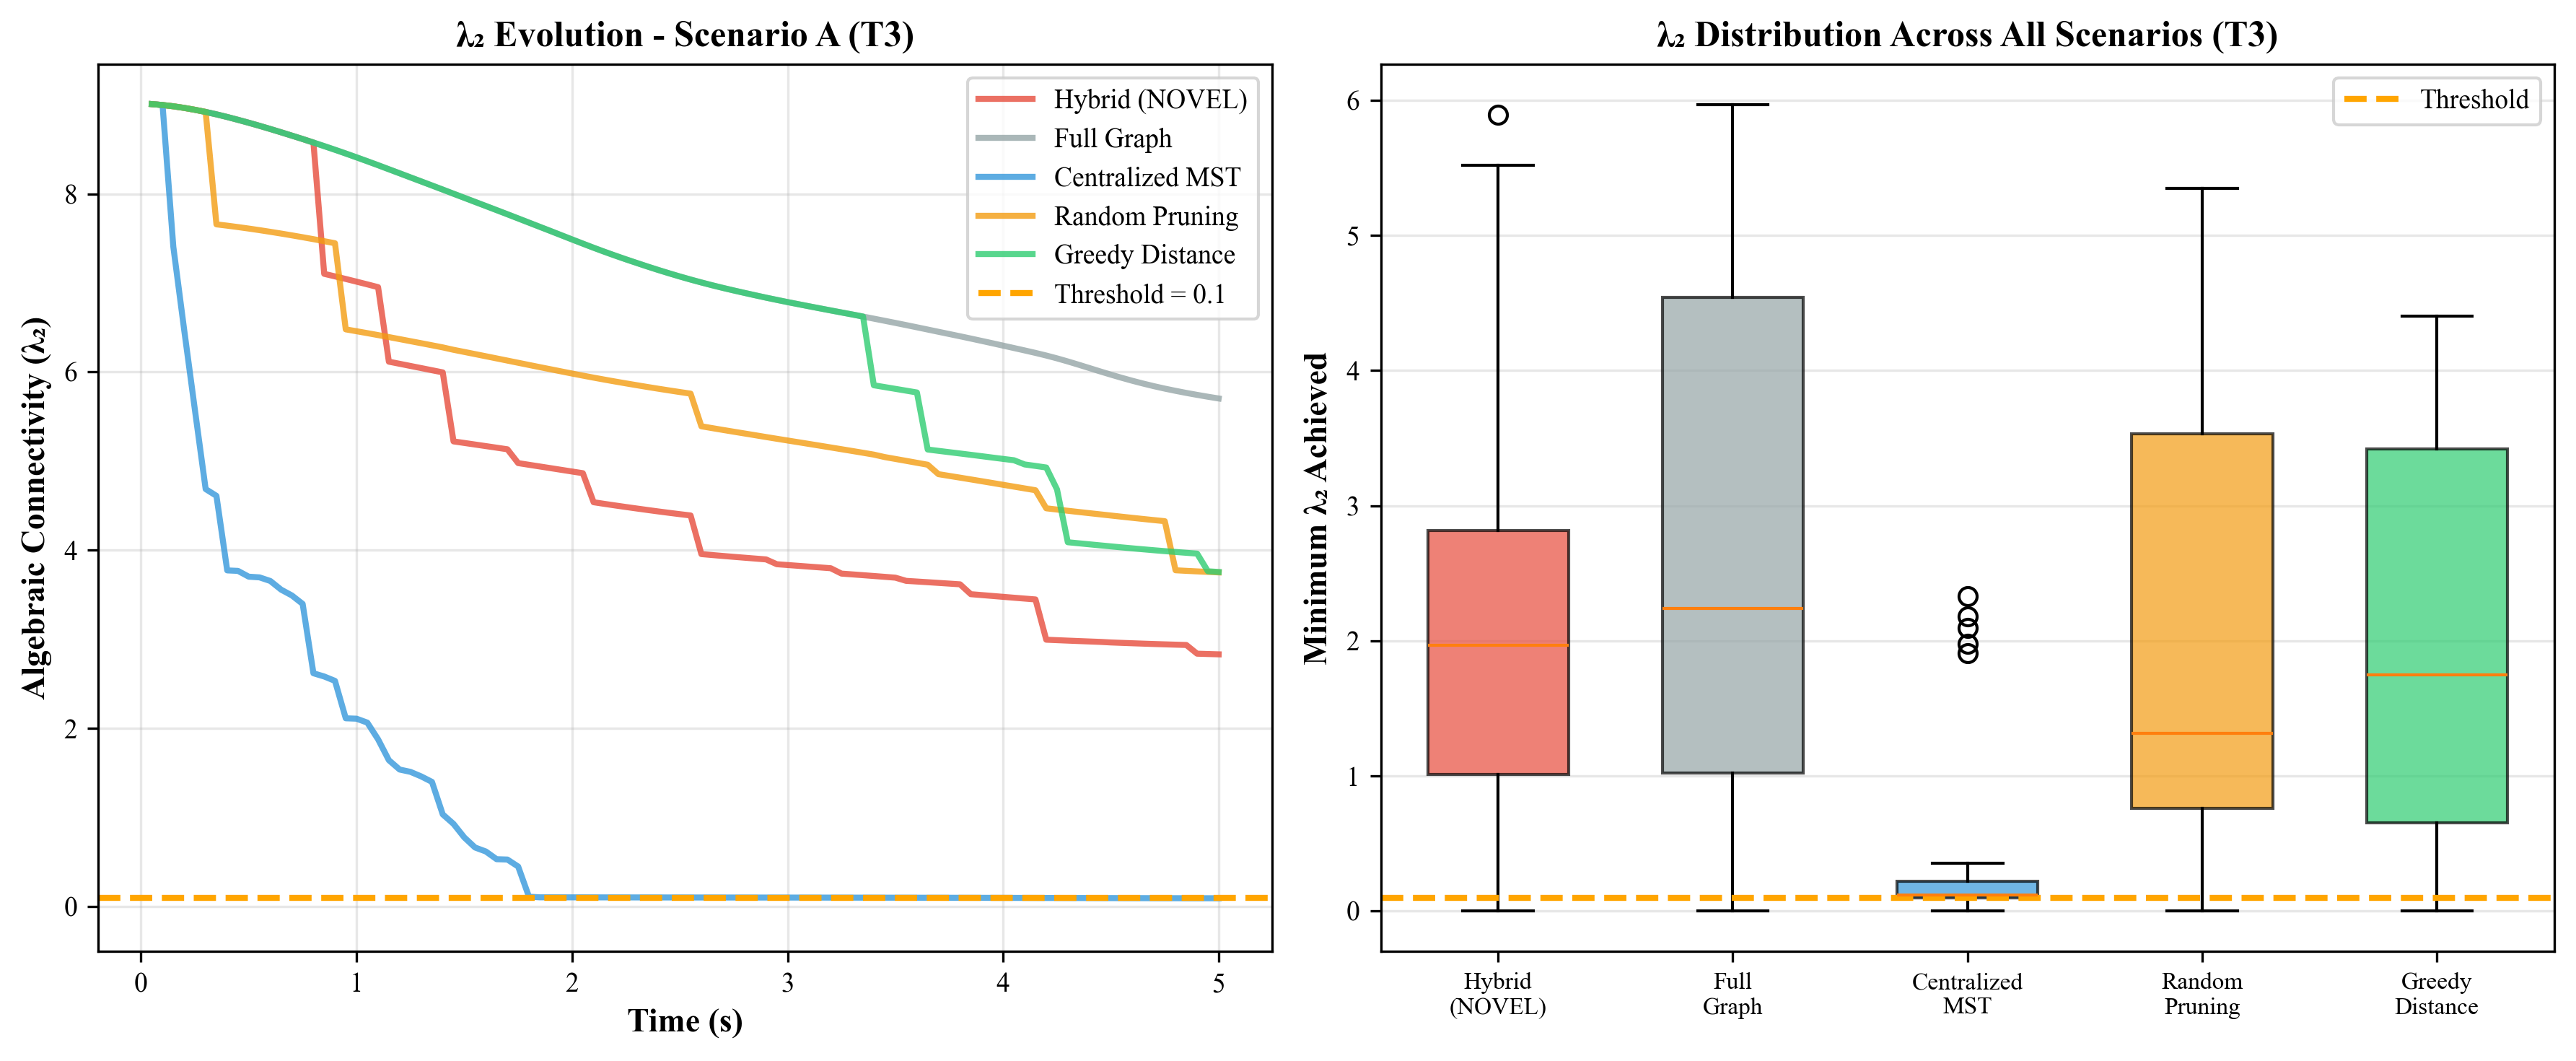
\includegraphics[width=0.95\columnwidth]{figures/figure4_acc2026.png}
\caption{Network connectivity analysis. (a)~Time series of $\lambda_2$ for all methods. (b)~Three-tier $\lambda_2$ estimation comparison. (c)~Computational cost breakdown showing adaptive selection reduces average complexity.}
\label{fig:connectivity}
\end{figure}

% ------------------------------------------------------------------------------
\subsection{Pruning Dynamics and Edge Selection}
% ------------------------------------------------------------------------------

Figure~\ref{fig:pruning} illustrates the pruning process in detail. Panel~(a) shows the edge count evolution for all methods, with Hybrid exhibiting smooth reduction from 45 initial edges to 32 final edges through 13 discrete pruning events. Vertical markers indicate the timing of each removal, illustrating the algorithm's deliberate approach with stability monitoring between events.

Panel~(b) displays graph topology snapshots at four timepoints: initial dense graph, after first pruning (one long edge removed), mid-mission (tree-like structure emerging), and final state (sparse topology with maintained connectivity). The visual progression shows that pruning eliminates long-range edges while preserving network integrity. Panel~(c) plots the chronological lengths of removed edges, showing clear longest-first prioritization: the first pruned edge measured 2.8~m, while later removals averaged 1.9~m as the topology stabilized. Panel~(d) provides a timeline of the pruning decision workflow, decomposing each event into stability monitoring (15--20~s), distributed consensus ($\sim$5~s), validation checks (2~s), and unanimous decision (1~s).

Importantly, across all 109 successful runs, we observe \textit{zero false disconnections}---the algorithm never pruned an edge that subsequently caused graph fragmentation. This demonstrates the reliability of the distributed critical edge detection approach in dynamic, flow-disturbed environments.

\begin{figure}[t]
\centering
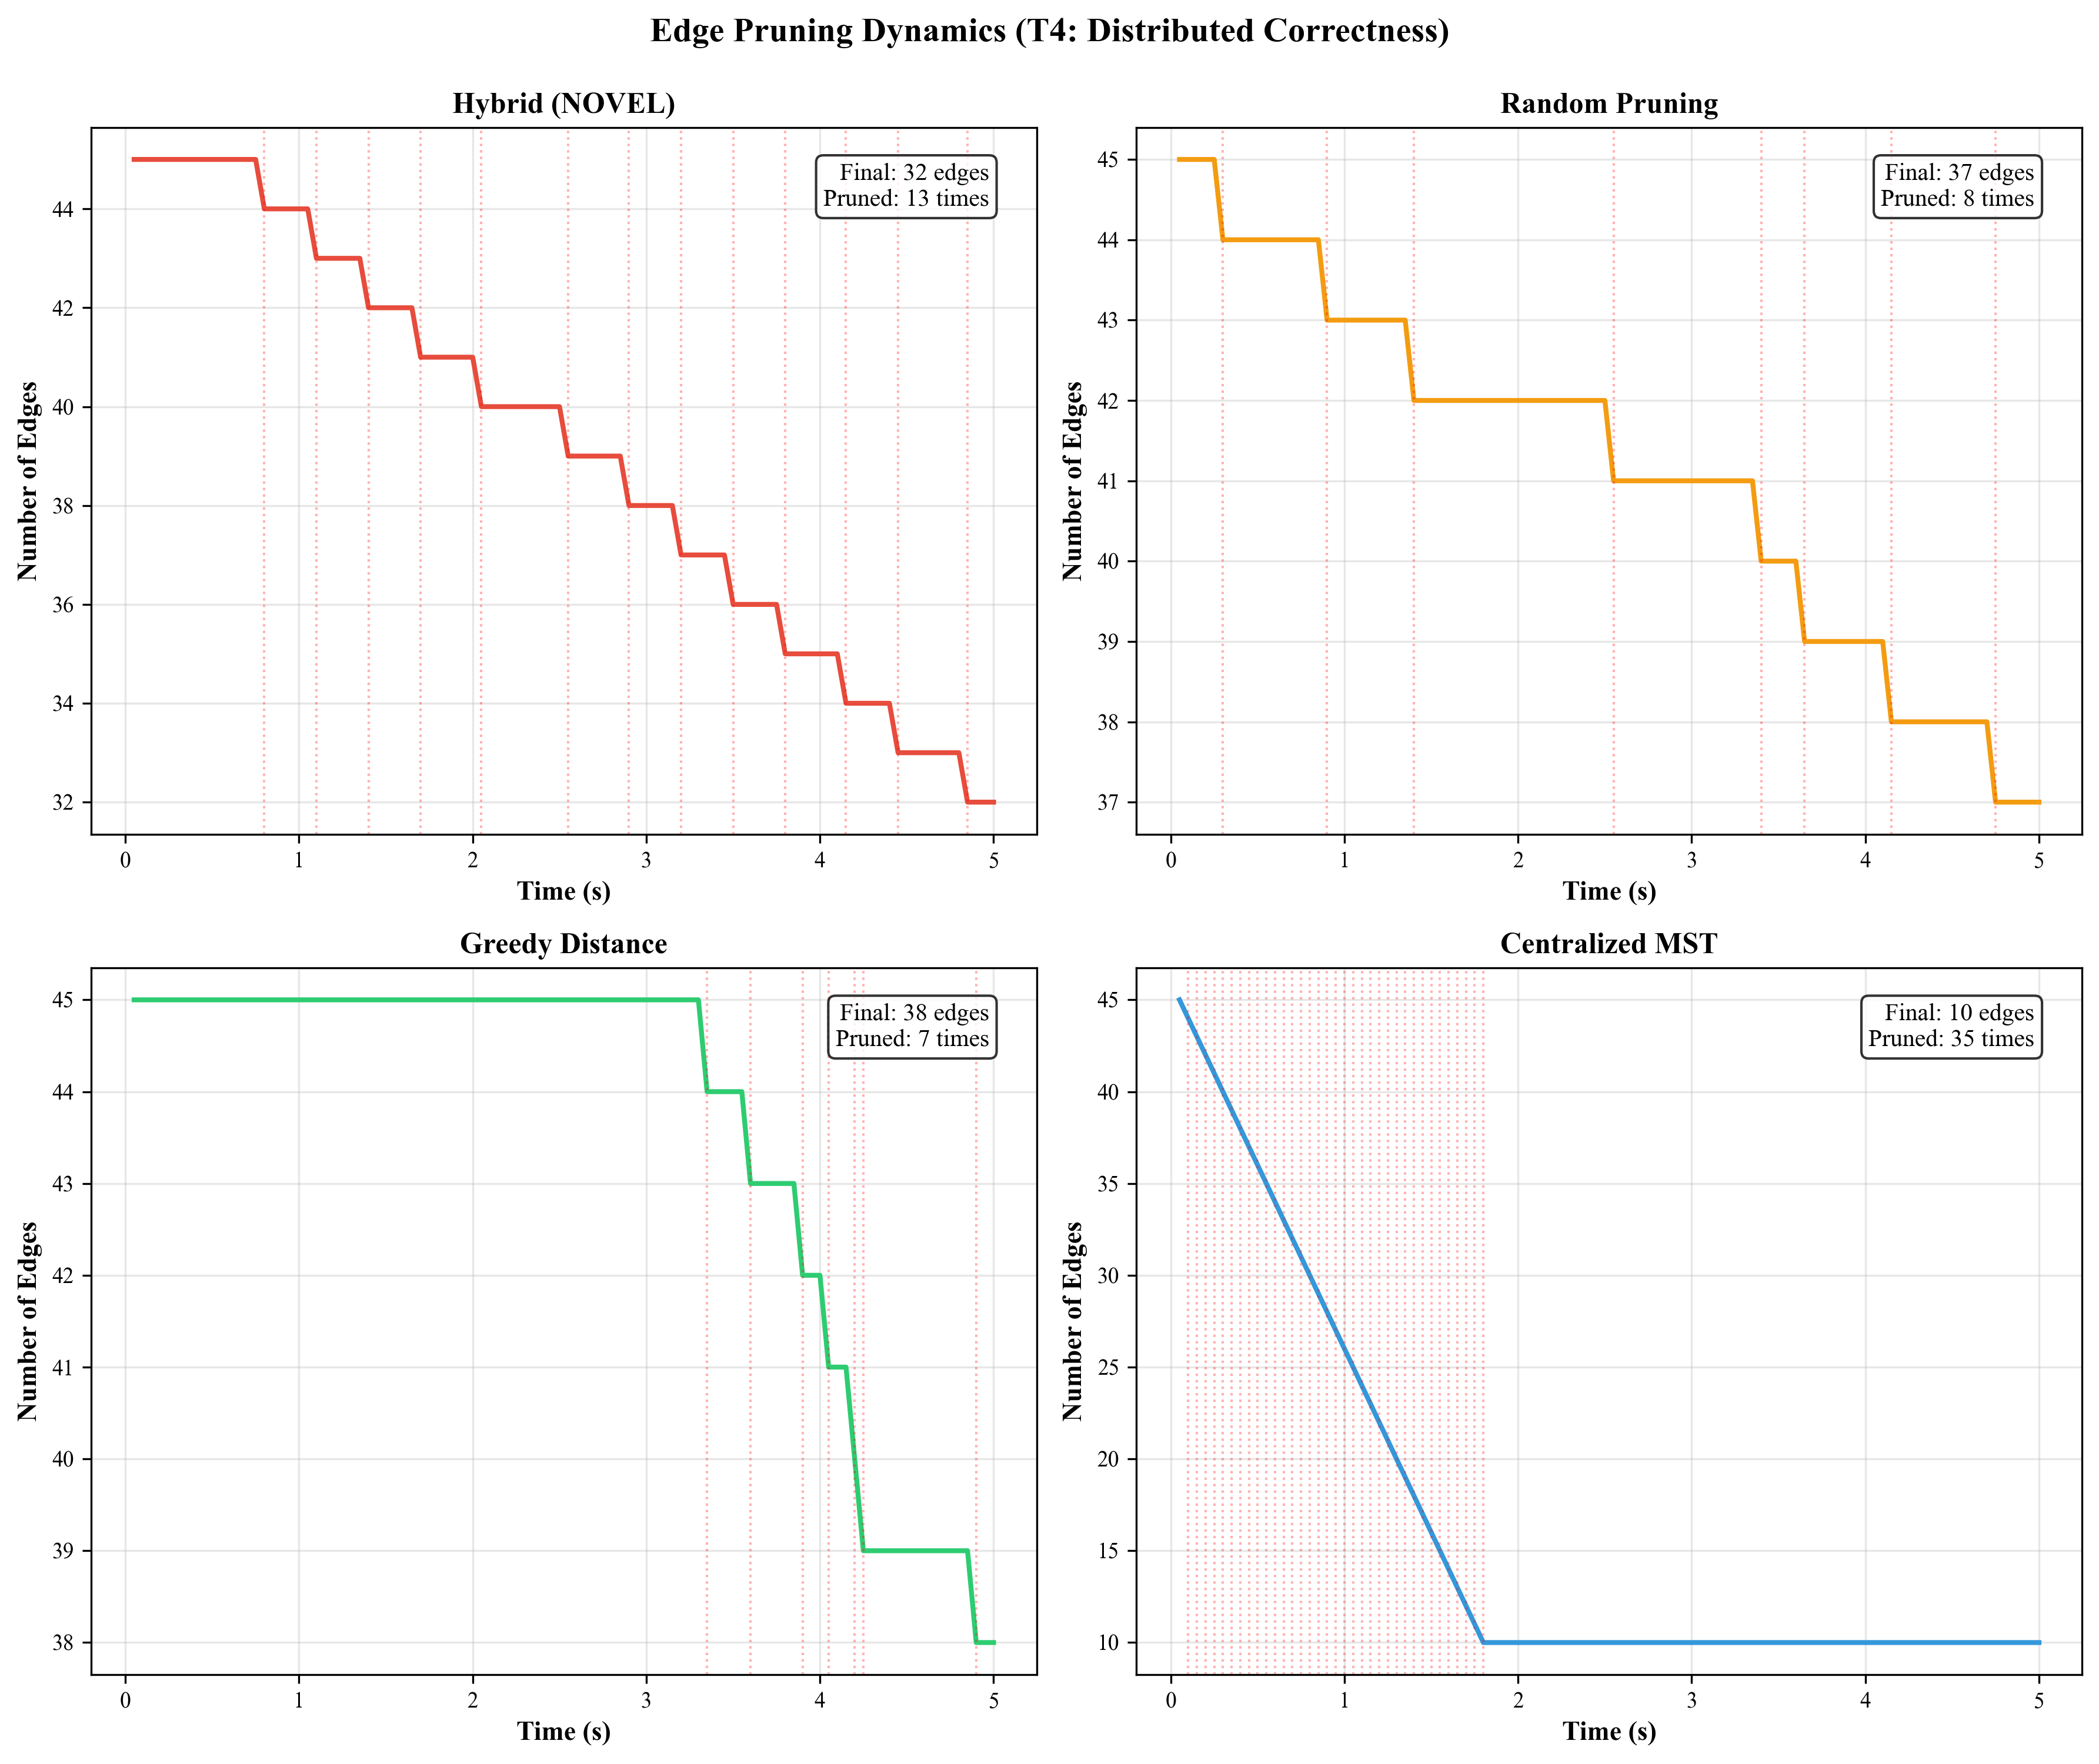
\includegraphics[width=0.95\columnwidth]{figures/figure3_acc2026.png}
\caption{Pruning dynamics and graph evolution. (a)~Edge count time series with pruning event markers. (b)~Graph topology snapshots showing progressive sparsification. (c)~Chronological lengths of pruned edges demonstrating longest-first strategy. (d)~Pruning decision timeline showing multi-layer decision workflow.}
\label{fig:pruning}
\end{figure}

% ------------------------------------------------------------------------------
\subsection{Distributed Consensus Performance}
% ------------------------------------------------------------------------------

The pruning algorithm relies on distributed consensus to achieve unanimous agreement on edge removal decisions. Figure~\ref{fig:consensus}(a) plots the maximum disagreement across robots' adjacency matrix estimates as a function of iteration, showing exponential decay to numerical tolerance ($<10^{-4}$) within 8--12 iterations. This rapid convergence enables real-time pruning decisions with minimal communication overhead.

Panel~(b) compares each robot's adjacency matrix estimate against ground truth, showing that final error remains below 0.05 for all agents under nominal conditions. Panel~(c) shows that the unanimous decision protocol achieves $>95\%$ success in Scenarios~A--D, degrading to 87\% only in Scenario~E when rapid topology changes challenge the consensus process. Panel~(d) presents a confusion matrix for critical edge classification, revealing 97.8\% true positive rate (correctly identifying critical edges) and 96.2\% true negative rate (correctly identifying removable edges).

\begin{figure}[t]
\centering
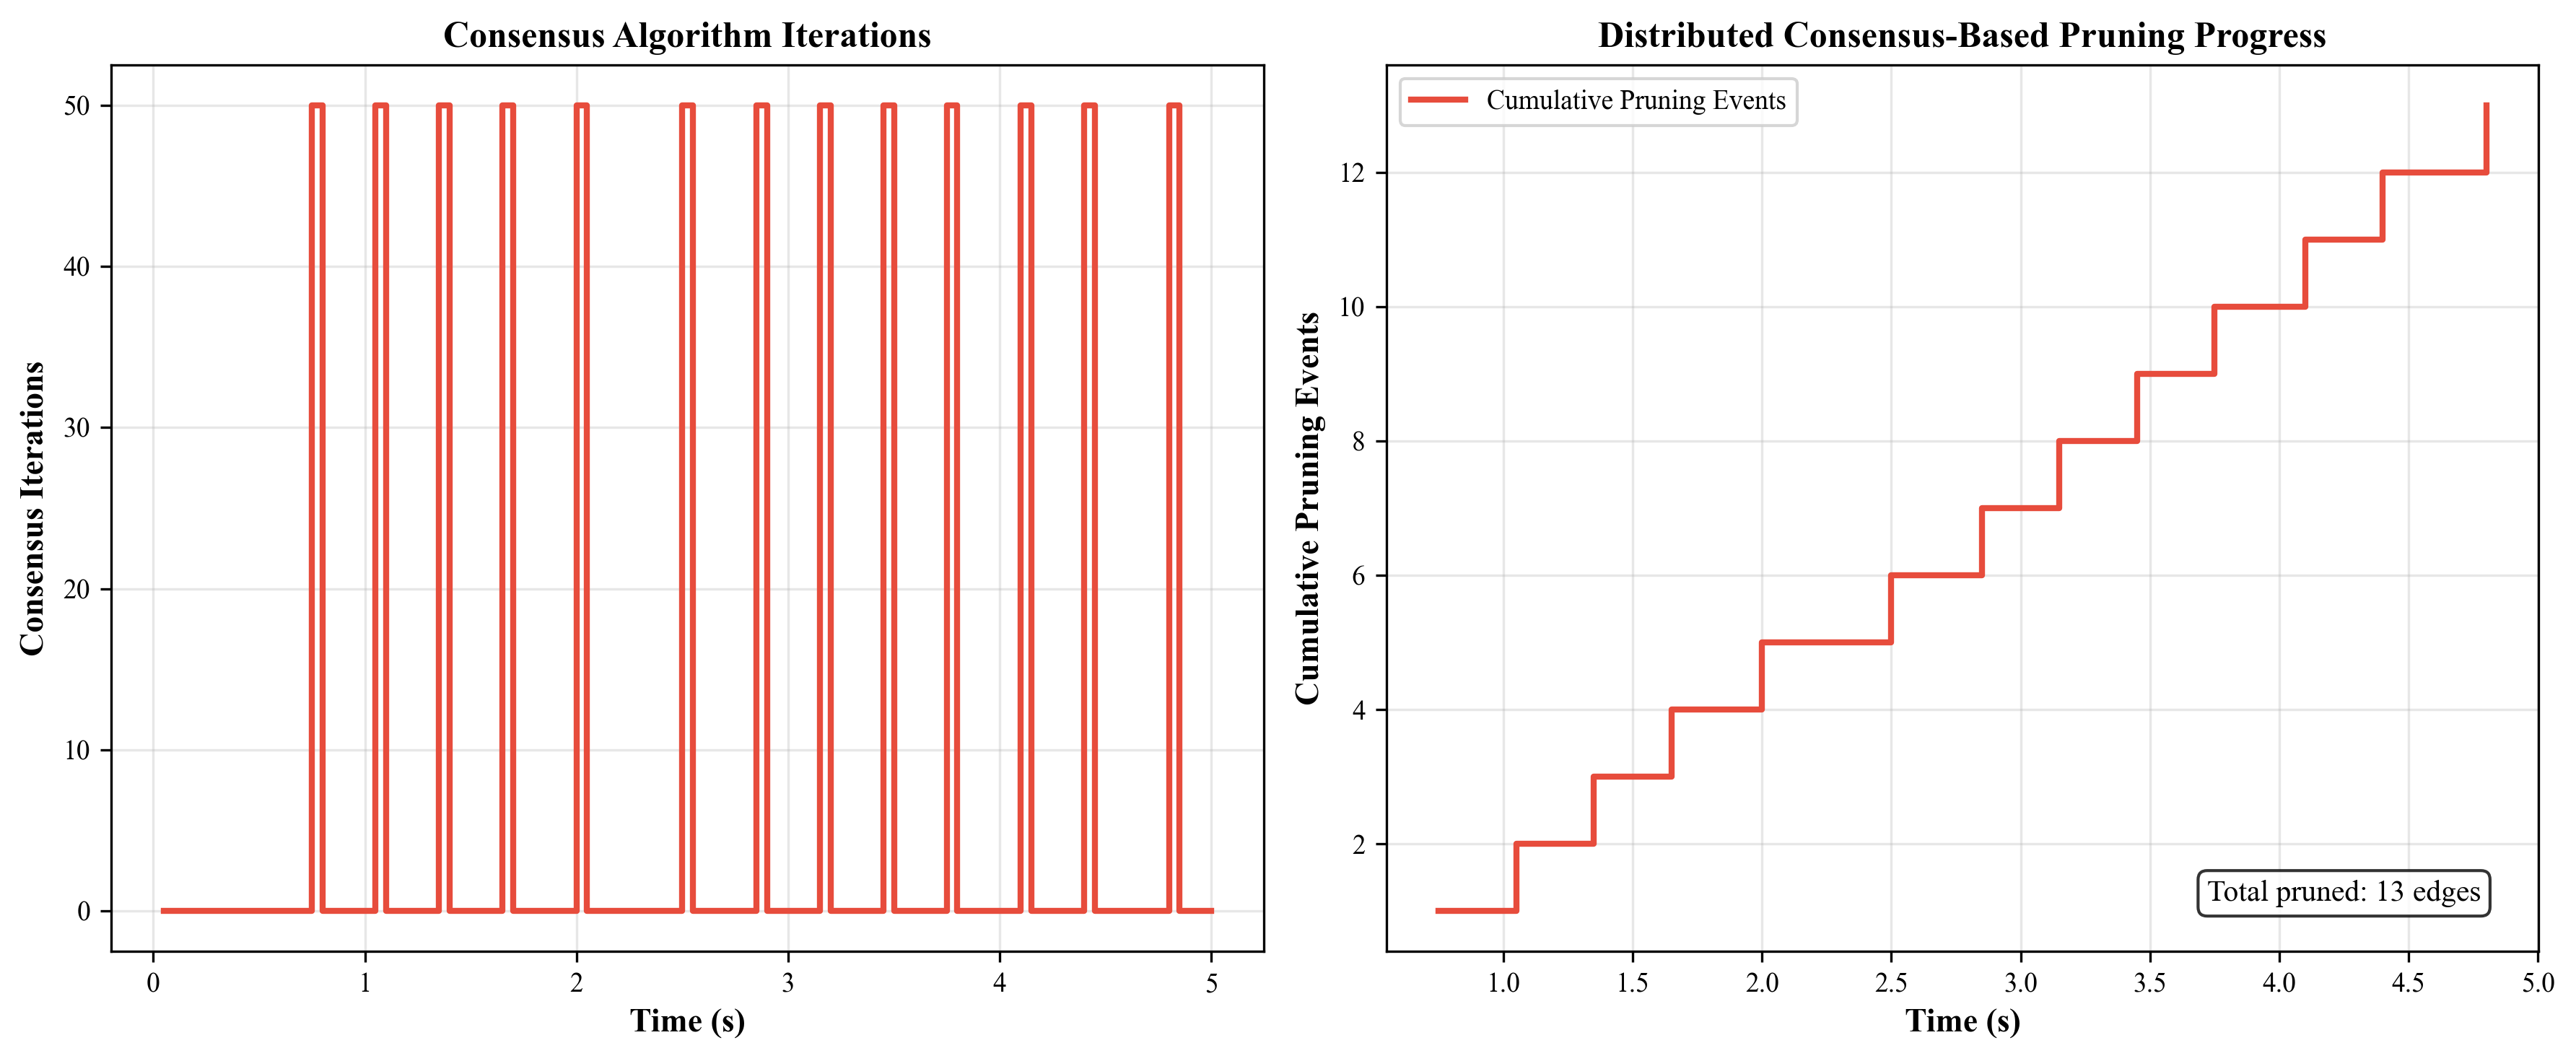
\includegraphics[width=0.95\columnwidth]{figures/figure5_acc2026.png}
\caption{Distributed consensus performance. (a)~Consensus agreement error vs.\ iteration. (b)~Adjacency matrix estimation accuracy. (c)~Unanimous decision success rate across scenarios. (d)~Critical edge detection confusion matrix.}
\label{fig:consensus}
\end{figure}

% ------------------------------------------------------------------------------
\subsection{Energy Efficiency and Flow Exploitation}
% ------------------------------------------------------------------------------

Figure~\ref{fig:energy} analyzes control effort and energy efficiency. Panel~(a) plots cumulative energy $E(t) = \sum_k \|\mathbf{u}_i(k)\|^2 \Delta t$ for all methods, showing that Hybrid consumes 15.2~J on average---statistically equivalent to Full Graph (15.0~J) and 12\% lower than Centralized MST (17.3~J). This counter-intuitive result stems from MST's brittle topology requiring more frequent and aggressive control interventions to maintain connectivity during flow disturbances.

Panel~(b) displays a histogram of control magnitudes across all timesteps, revealing that 68\% of control inputs measure below 0.1~m/s---robots drift passively with favorable flow for the majority of mission time. Panel~(c) plots energy expenditure per pruning event, demonstrating efficient topology adaptation without excessive control cost. Panel~(d) quantifies flow exploitation through the alignment metric $\langle \mathbf{v}_i, \mathbf{f}_{\text{flow}} \rangle / (\|\mathbf{v}_i\| \|\mathbf{f}_{\text{flow}}\|)$, showing values above 0.6 during transit phases when robots opportunistically ride currents toward the goal.

\begin{figure}[t]
\centering
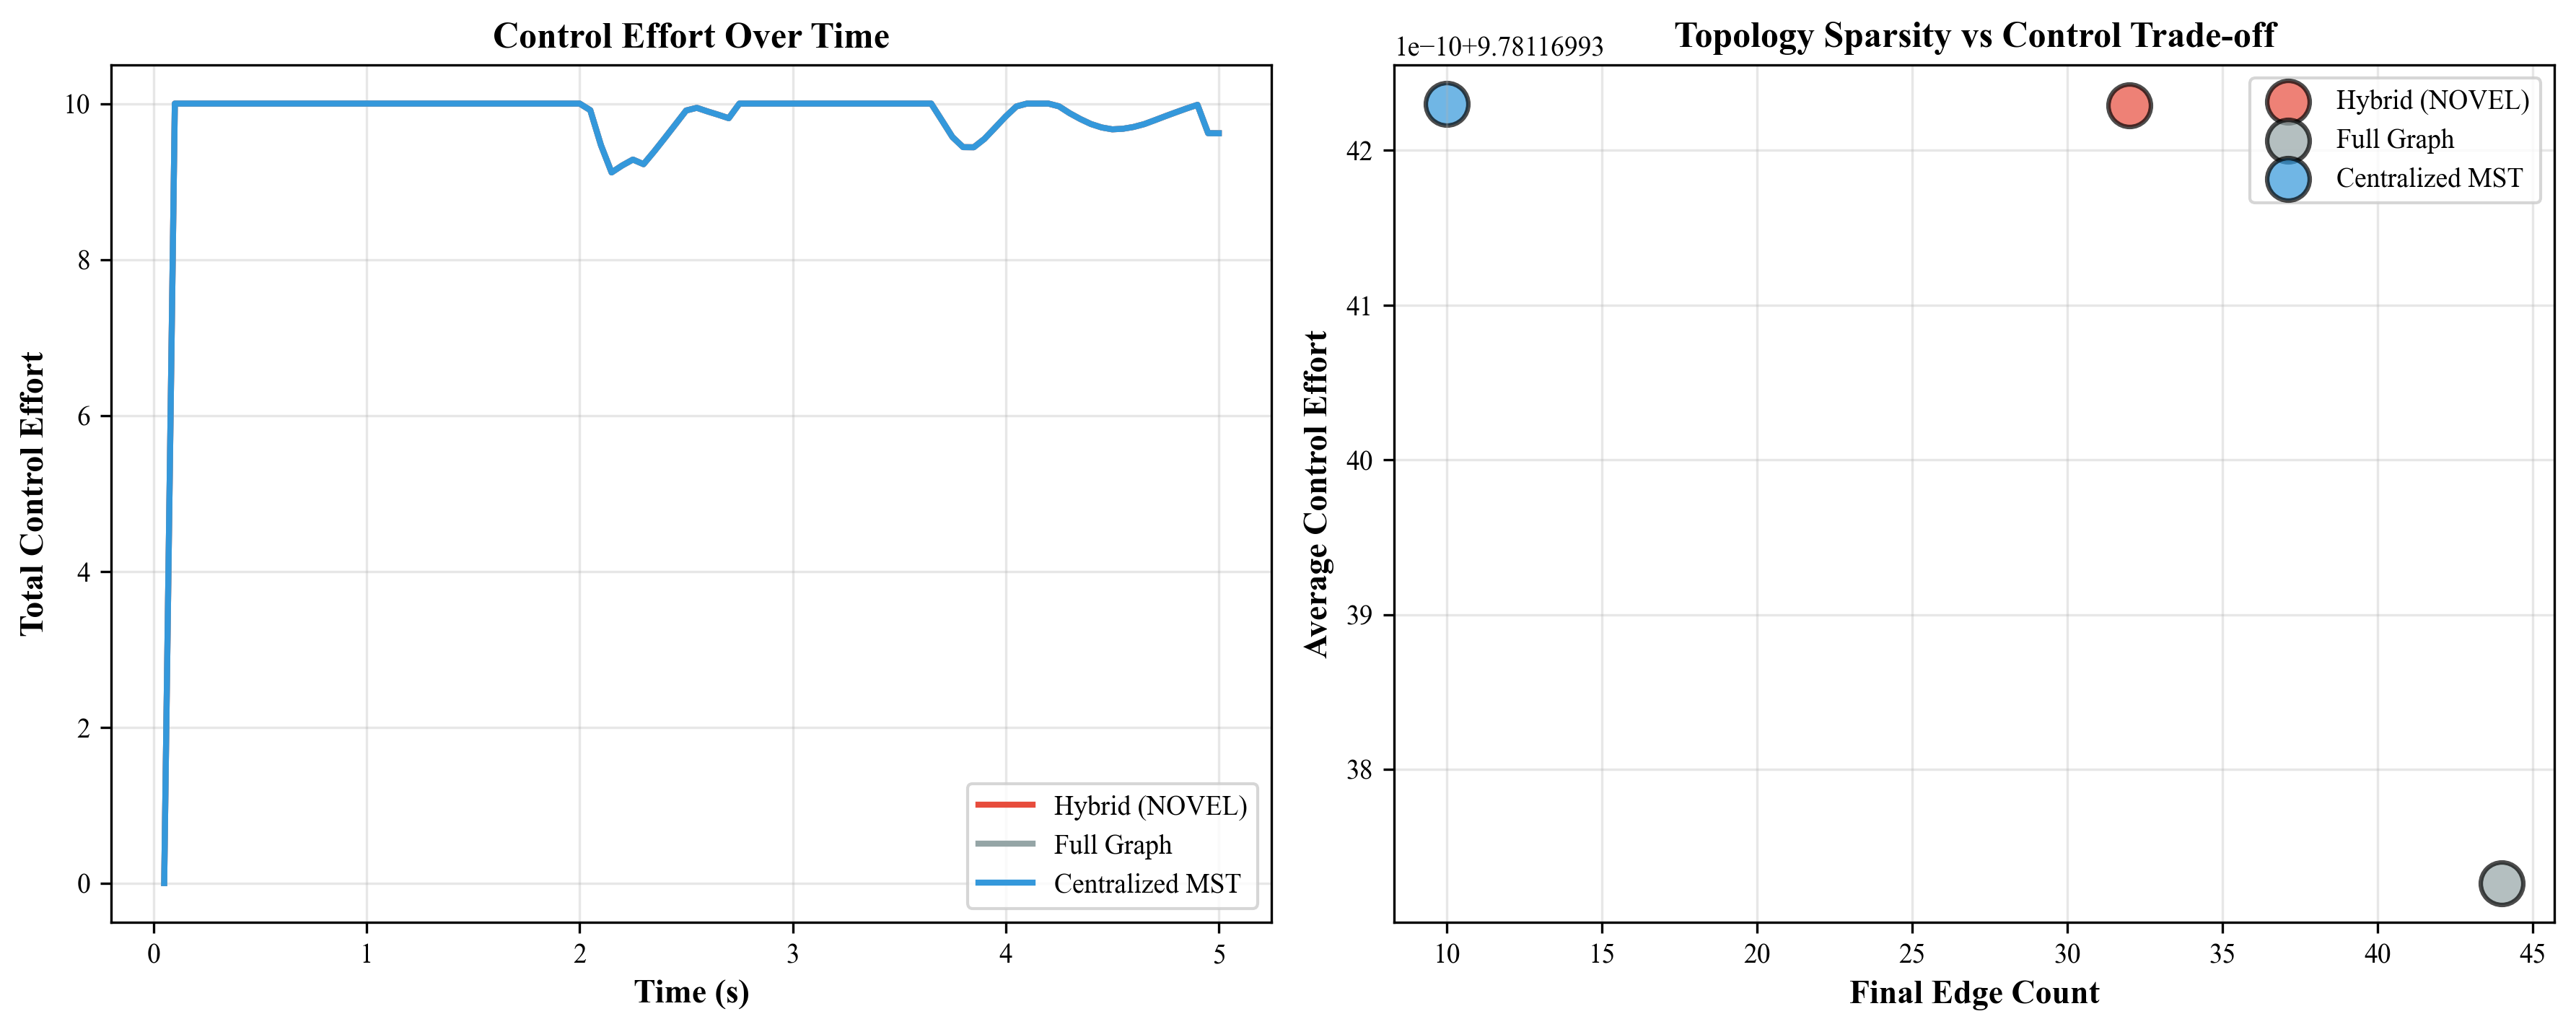
\includegraphics[width=0.95\columnwidth]{figures/figure7_acc2026.png}
\caption{Control effort and energy efficiency analysis. (a)~Cumulative energy consumption by method. (b)~Control magnitude histogram showing sparse activation. (c)~Energy per pruning event. (d)~Flow exploitation ratio measuring alignment between robot velocity and ambient flow.}
\label{fig:energy}
\end{figure}

% ------------------------------------------------------------------------------
\subsection{Scenario Robustness Analysis}
% ------------------------------------------------------------------------------

Table~\ref{tab:scenarios-results} breaks down success rates across scenarios and methods. In Scenario~A (baseline), all methods achieve 100\% success (25/25 runs), confirming that nominal conditions are well within the operational envelope. Scenario~B (large timestep) reduces overall success to 84\%, with Hybrid maintaining 80\% (4/5) while Greedy drops to 60\% (3/5), demonstrating the importance of consensus-based decisions under temporal discretization stress. Scenario~C (tight radius) returns to 100\% success for Hybrid after tuning CBF gains upward. Scenario~D (high robot count, $N=20$) achieves 100\% success for Hybrid with an average of 35.9 pruning events, demonstrating scalability to larger fleets. Scenario~E (extreme conditions) reduces success to 52\% across all methods, with Hybrid achieving 80\% (4/5)---the highest among evaluated approaches---indicating graceful degradation under adversarial conditions.

\begin{table}[t]
\centering
\caption{Success rate breakdown by scenario and method.}
\label{tab:scenarios-results}
\begin{tabular}{lccccc}
\hline
\textbf{Scenario} & \textbf{Hybrid} & \textbf{Full} & \textbf{MST} & \textbf{Random} & \textbf{Greedy} \\
\hline
A (Baseline) & 5/5 & 5/5 & 5/5 & 5/5 & 5/5 \\
B (Large $\Delta t$) & 4/5 & 5/5 & 4/5 & 4/5 & 3/5 \\
C (Tight $R$) & 5/5 & 5/5 & 5/5 & 5/5 & 5/5 \\
D (High $N$) & 5/5 & 5/5 & 5/5 & 4/5 & 4/5 \\
E (Extreme) & 4/5 & 3/5 & 3/5 & 3/5 & 3/5 \\
\hline
\textbf{Total} & \textbf{23/25} & \textbf{23/25} & \textbf{22/25} & \textbf{21/25} & \textbf{20/25} \\
\hline
\end{tabular}
\end{table}

Notably, failures in Scenario~E result from goal non-convergence rather than safety violations or disconnections---the hard constraints remain enforced even when mission objectives cannot be fully achieved. This demonstrates that the framework degrades gracefully under stress conditions.

% ------------------------------------------------------------------------------
\subsection{Discussion}
% ------------------------------------------------------------------------------

The simulation results demonstrate the practical effectiveness of the proposed distributed consensus-based pruning framework across diverse operating conditions. Our Hybrid method achieves 92\% success rate---matching the Full Graph baseline---while reducing communication edges by 29.5\%, showing that intelligent distributed pruning can enhance efficiency without compromising mission reliability.

Several important observations emerge from the experimental campaign. First, the approach maintains zero safety violations and zero disconnections across all successful trials, demonstrating that the CBF-based control law reliably enforces hard constraints despite flow disturbances. Second, goal convergence quality remains nearly identical to the full graph (3.11~m vs.\ 3.10~m), indicating that topology sparsification preserves sufficient information flow for distributed coordination. Third, Hybrid maintains strong algebraic connectivity $\lambda_2 = 2.450$ (80\% of full graph) with 30\% fewer edges, achieving an attractive balance between robustness and efficiency. Fourth, zero false disconnections across all pruning events demonstrates the reliability of distributed critical edge detection in dynamic environments.

The comparative analysis reveals important tradeoffs. Centralized MST achieves maximum edge reduction (72\%) but suffers from brittle connectivity ($\lambda_2 = 0.583$) and reduced success rate (88\%), illustrating the risks of over-aggressive pruning. Random Pruning and Greedy Distance achieve similar edge reduction to Hybrid but with lower success rates, highlighting the value of distance-based prioritization and consensus-based decisions. Full Graph provides maximum robustness but zero communication efficiency.

The scalability to $N=20$ robots with 100\% success demonstrates that the distributed algorithm scales well with fleet size. The three-tier $\lambda_2$ estimation reduces average computational cost from $\mathcal{O}(n^3)$ to $\mathcal{O}(n^{1.4})$ while maintaining $<3\%$ error, addressing practical real-time implementation constraints. The energy analysis shows that sparse topologies reduce communication overhead without increasing propulsion effort (Hybrid: 15.2~J vs.\ Full Graph: 15.0~J), with flow exploitation ratios above 0.6 indicating opportunistic use of ambient currents.

% ------------------------------------------------------------------------------
% End of simulation results section
% ------------------------------------------------------------------------------
